%\hypertarget{aula-13}{%
%\chapter{Aula: 13}\label{aula-13}}




\hypertarget{ip-o-protocolo-da-network-layer}{%
\chapter{IP, o protocolo da Network Layer}\label{ip-o-protocolo-da-network-layer}}

O objetivo da \emph{network layer} (camada de rede) é transferir dados
de um \emph{host} emissor para o \emph{host} receptor (como não há
garantias, esse serviço é conhecido como \emph{best-effort service}).
Para tal, é necessário determinar a rota (\emph{route} ou \emph{path})
global que os dados devem pecorrer para alcançar o seu destino, chamado
de \emph{routing}, bem como especificar o caminho local com o
direcionamento dos dados recém chegados no roteador para a sua saída
apropriada, chamado de \emph{fowarding}.

Dessa forma, a \emph{network layer} pode ser decomposta em duas partes,
\emph{control plane} e \emph{data plane}, nas quais estão contidos o
\emph{routing} e o \emph{fowarding}, como mostrado na Figura \ref{Control plane e data plane}.

\begin{figure}[h!]
\centering
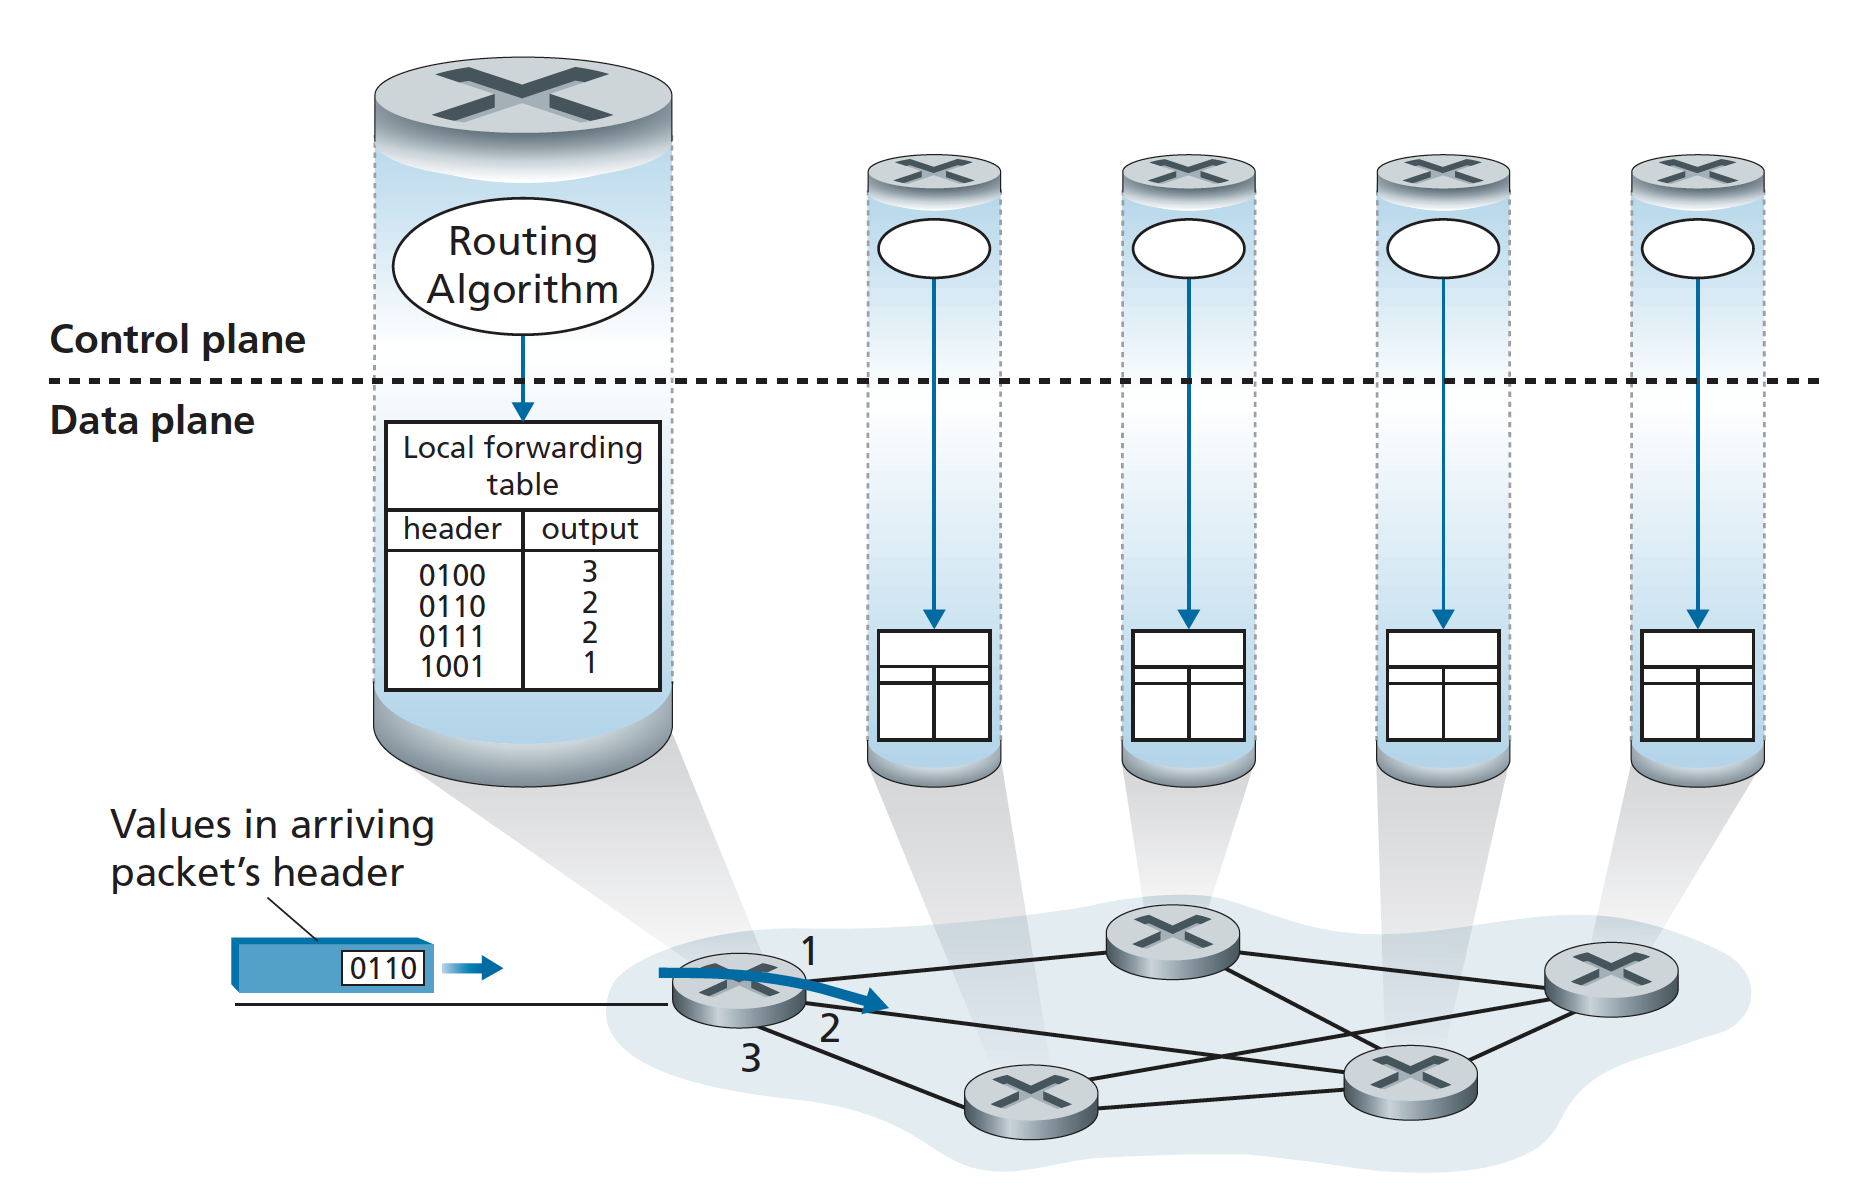
\includegraphics[keepaspectratio, width=15cm, height=12cm]{imagens/13/13 - Control plane and data plane.png}
\caption{Control plane e data plane \\
Imagem retirada de: Computer Networking a top-down approach. 8th
ed.~Pearson, página 307. \\}
\label{Control plane e data plane}
\end{figure}



É importante perceber que apesar dessas duas funcionalidades serem
requisitos para a \emph{network layer}, é possível encontrá-las em
dispositivos separados, algo possibilitado pelo SDN (Software-Defined
Networks), que aloca o \emph{control plane} em um servidor, algo que
torna os roteadores especialistas em \emph{fowarding}.

A \emph{fowarding table}, responsável por determinar, a partir do
\emph{header} dos dados recebidos pelo roteador, a saída apropriada, é o
elemento chave para a interação entre essas partes (\emph{control plane}
e \emph{data plane}), pois seus registros são gerados pelo \emph{control
plane} e utilizados pelo \emph{data plane}.

\hypertarget{protocolo-ip}{%
\section{Protocolo IP}\label{protocolo-ip}}

O IP (\emph{Internet Protocol}) é o protocolo utilizado na camada de
rede. Atualmente está largamente em uso as versões 4 e 6, as quais serão
discutidas a seguir. A estrutura de dados resultante da \emph{network
layer} é o \emph{datagram}, no qual o seu arranjo varia conforme a
versão utilizada.

Citando o livro-texto desse curso:

``Nevertheless, the datagram plays a central role in the internet -
every networking student and professional needs to see it, absorb it,
and master it.'' (Computer Networking a top-down approach. 8th
ed.~Pearson, página 331)

Entender o \emph{datagram} é de suma importância para a aprendizagem de
redes de computadores.

\hypertarget{ipv4-datagram}{%
\section{IPv4 Datagram}\label{ipv4-datagram}}

O \emph{datagram}, como mostrado na Figura \ref{IPv4 Datagra }, segue o seguinte formato:

\begin{enumerate}
\def\labelenumi{\arabic{enumi}.}

\item
  Version Number: especifica a versão utilizada (no caso, 4)
\item
  Header length: a versão 4 do IP tem um tamanho de \emph{header}
  variável, causado pelo campo \emph{options}, o que torna necessário a
  manutenção dessa informação dentro do \emph{datagram} (o campo
  \emph{options} não é normalmente utilizado, portanto o tamanho típico
  do \emph{header} IPv4 \emph{datagram} é de 20 \emph{bytes})
\item
  Type of Service (TOS): exemplos são \emph{real time},
  \emph{non-real-time}.
\item
  Datagram length: o tamanho do \emph{datagram} é calculado pela soma
  dos tamanhos do header dos dados carregados (\emph{payload}). Composto
  por 16 bits e medido em \emph{bytes}, o tamanho teórico máximo é de
  65535 bytes (raramente ultrapassa os 1500 bytes).
\item
  Identifier, flags e fragmentation offset: utilizados para fragmentar
  um \emph{datagram} muito grande em pedaços pequenos que serão enviados
  independentemente e remontados no destino.
\item
  time-to-live (ttl): decrementa em 1 toda vez que o \emph{datagram} é
  processado por um roteador, sendo descartado ao atingir 0.
\item
  Protocol: indica o protocolo da camada de transporte. contém o valor
  de 6 (00110) para TCP e 17 (10001) para UDP.
\item
  Header Checksum: Objetivando detectar erros, esse campo é computado
  tratando cada 2 bytes do \textbf{header} como um número e somando-os
  utilizando a aritmética complementar de 1. Esse cáculo é somente feito
  para o \textbf{header}, evitando possíveis redundâncias com as camadas
  inferiores.
\item
  Source e destination IP addresses.
\item
  Options: permite uma extensão do \emph{header}. Não foi incluido no
  \emph{datagram} do IPv6 por dificultar a determinação do início do
  \emph{payload} (necessitando do campo \emph{header length}) e a
  variação do tempo requerido para processamento (pois alguns
  \emph{datagrams} podem requisitar ou não o processamento do campo
  \emph{options}).
\item
  Data (payload): contém o segmento da camada de transporte.
\end{enumerate}



\begin{figure}[h!]
\centering
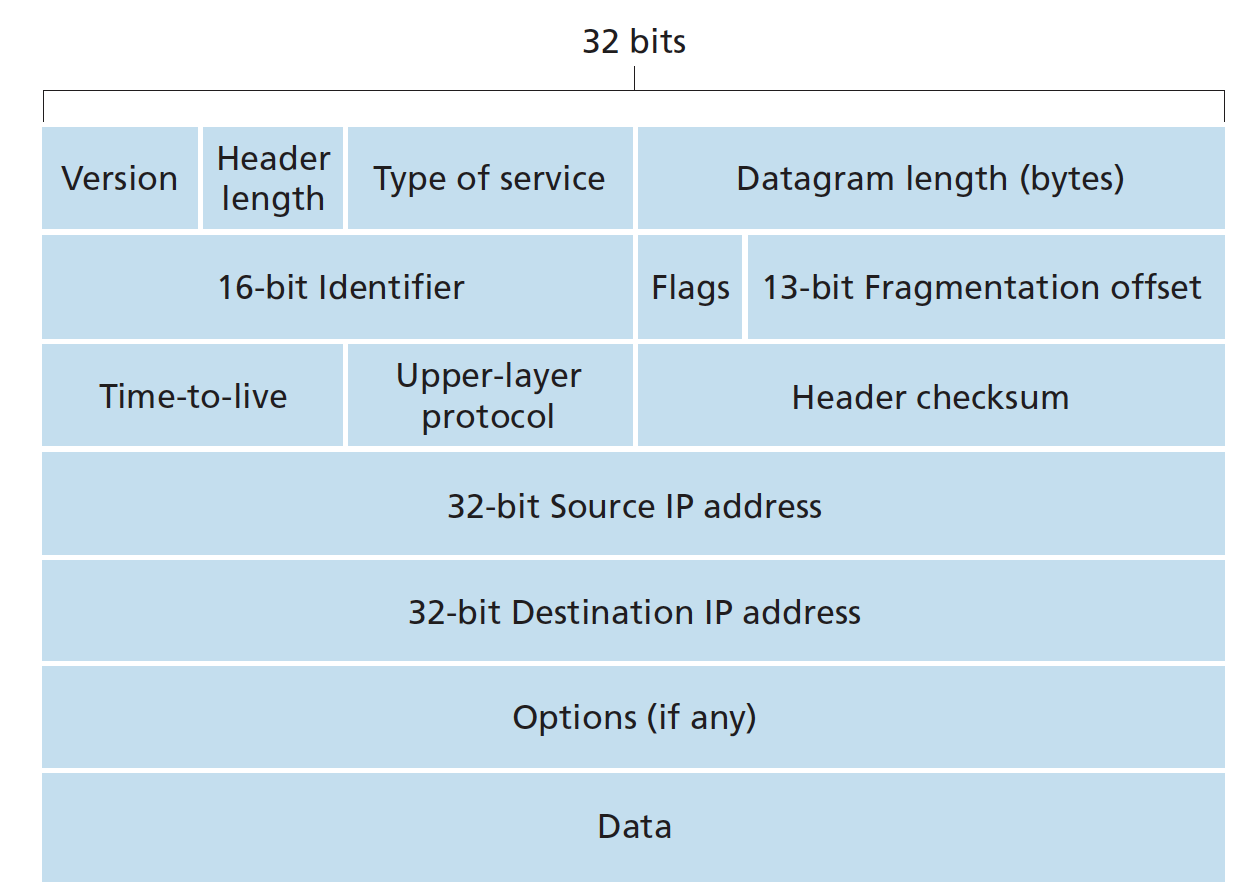
\includegraphics[keepaspectratio, width=12cm, height=9cm]{imagens/13/13 - IPv4 Datagram.png}
\caption{IPv4 Datagra \\
Imagem retirada de: Computer Networking a top-down approach. 8th
ed.~Pearson, página 331. \\}
\label{IPv4 Datagra }
\end{figure}





\hypertarget{endereuxe7amento}{%
\section{Endereçamento}\label{endereuxe7amento}}

A fronteira entre o \emph{host} e a conexão física é chamada de
interface. Em um roteador é possível identificar múltiplas interfaces.
Como cada interface está associado um endereço de IP, um roteador,
portanto, pode estar associado a múltiplos endereços de IP. O endereço
de IP é formado por 4 bytes (32 bits), escritos na notação
\emph{dotted-decimal}, no qual cada byte é escrito em decimal e separado
por um ponto.

O endereçamento segue a estratégia conhecida como \emph{Classless
Interdomain Routing} (CIDR), no qual o endereço de IP (formado por 32
bits) é separado em prefixo (os \texttt{x} primeiros bits) e
identificador de host (os restantes \texttt{32\ -\ x} bits). O número de
bits (\texttt{x}) que formam o prefixo é determinado pela máscara de
rede (\emph{mask subnet}), como mostrado a seguir:

\begin{verbatim}
Endereço de IP: a.b.c.d
Endereço de IP com máscara de rede: a.b.c.d/x
Notação: 193.32.216.9/24 (11000001 00100000 11011000 00001001)
Prefixo (Sub-rede): 193.32.216 (11000001 00100000 11011000)
Identificador de Host: 9 (00001001)
\end{verbatim}

A máscara de sub-rede (\emph{network mask}) distingue o endereço
referente à sub-rede ao do \emph{host}. A sub-rede pode ser entendida como
uma ilha de rede isolada, com as interfaces compondo as bordas dessa
rede, como mostrado na Figura \ref{Subrede}.


\begin{figure}[h!]
\centering
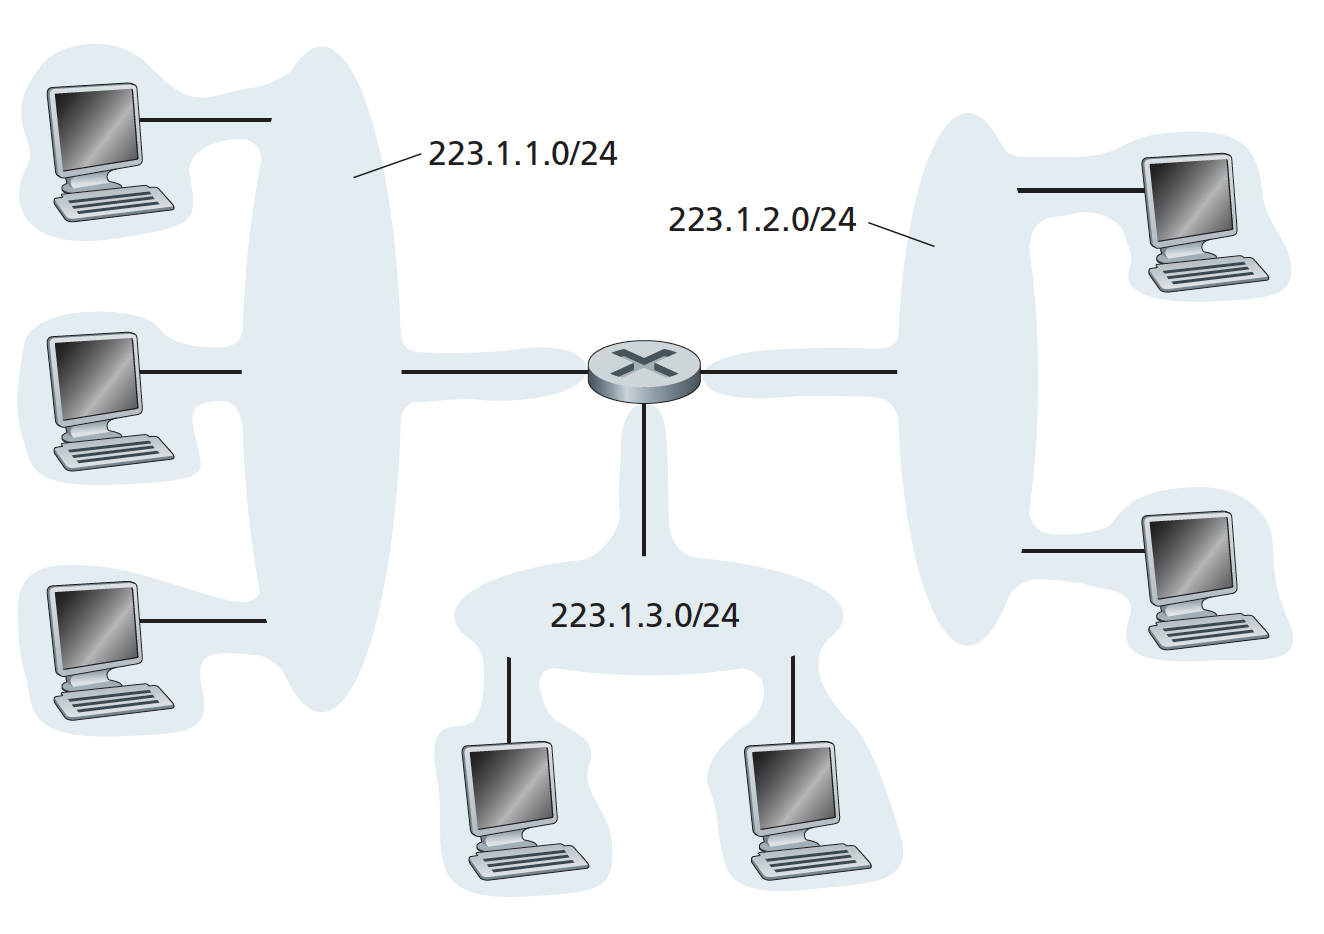
\includegraphics[keepaspectratio, width=12cm, height=9cm]{imagens/13/13 - subnet.png}
\caption{Sub-rede \\
Imagem retirada de: Computer Networking a top-down approach. 8th
ed.~Pearson, página 336. \\}
\label{Subrede}
\end{figure}





\hypertarget{obter-um-endereuxe7o-de-ip}{%
\subparagraph{Obter um endereço de
IP}\label{obter-um-endereuxe7o-de-ip}}

A obtenção de um endereço de IP ocorre de forma automática com o
protocolo DHCP (\emph{Dynamic Host Configuration Protocol}), chamado
também de protocolo \emph{plug-and-play} ou \emph{zeroconf} (\emph{zero
configuration}), o qual gera um endereço de IP temporário diferente toda
vez que o \emph{host} conecta-se nessa rede. O DHCP é um protocolo
baseado na arquitetura \emph{client-server}, e o seu processo é feito em
quatro passos (mostrado na Figura \ref{Processo DHCP }):

\begin{enumerate}
\def\labelenumi{\arabic{enumi}.}
\tightlist
\item
  Server Discovery: o \emph{client} dispara \emph{datagram} contendo um
  \emph{discovery message} para o destino 255.255.255.255 (esse endereço
  de IP indica ao roteador que a mensagem deva ser entregue para todos
  as interfaces da sub-rede), com a origem em 0.0.0.0.
\item
  Server Offer: O Servidor DHCP, após receber a discovery message\emph{,
  responde com a }offer message* para 255.255.255.255 (ou seja,
  disparando para todos os dispositivos da subrede). A \emph{offer
  message} contém: uma proposta de \emph{IP address}; \emph{network
  mask}; e o \emph{IP address lease time}, referente à validade do IP. É
  importante perceber que na mesma rede pode haver múltiplos servidores
  DHCP e, portanto, múltiplas \emph{offer message} podem ser disparadas
  durante essa etapa.
\item
  Request: o \emph{client} escolhe uma \emph{server offer} e ecoa os
  seus parâmetros com a \emph{request message}.
\item
  ACK: o servidor selecionado confirma a seleção do endereço enviando
  uma \emph{ACK message}.
\end{enumerate}


\begin{figure}[h!]
\centering
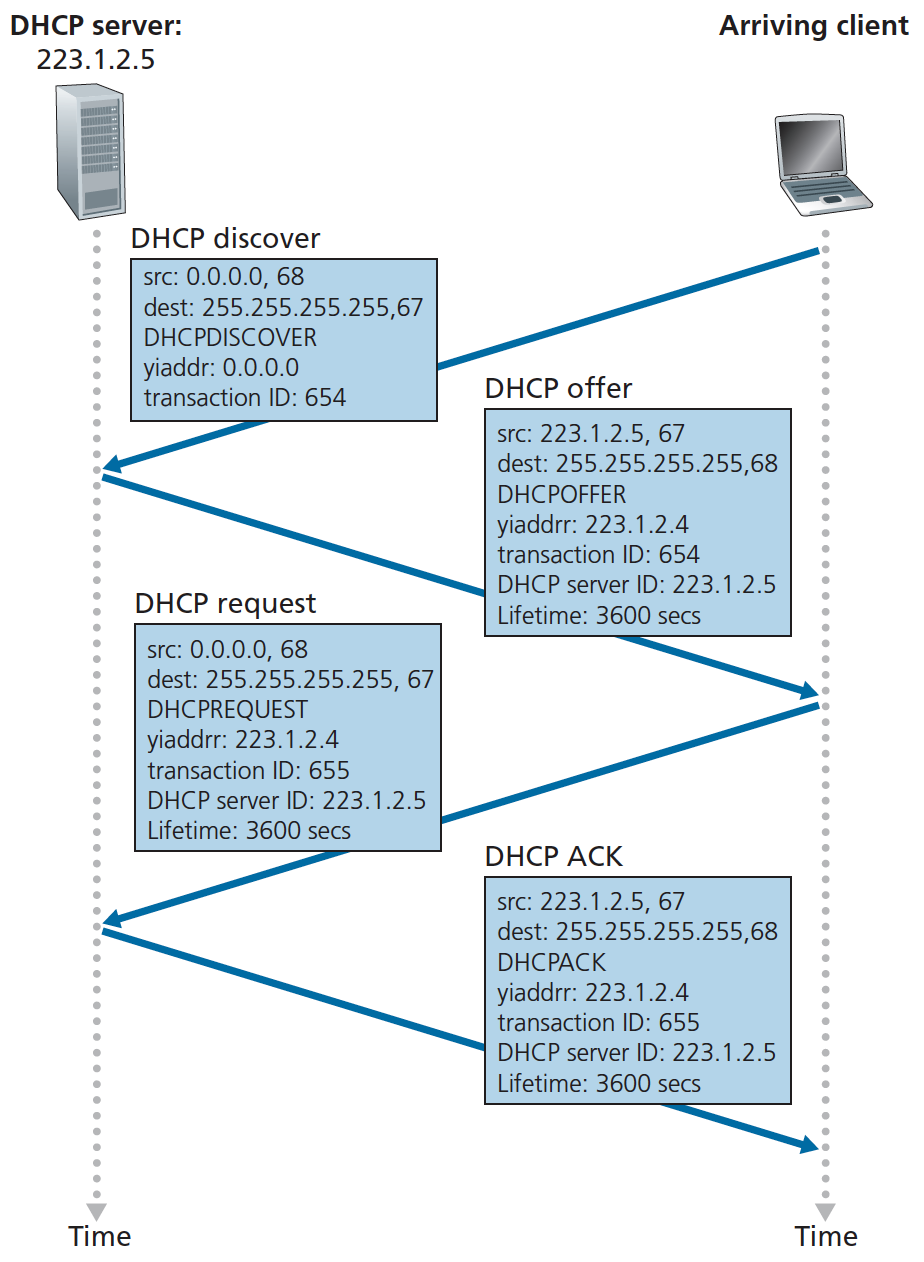
\includegraphics[keepaspectratio, width=18cm, height=15cm]{imagens/13/13 - DHCP process.png}
\caption{Processo DHCP \\
Imagem retirada de: Computer Networking a top-down approach. 8th
ed.~Pearson, página 343. \\}
\label{Processo DHCP }
\end{figure}


\hypertarget{nat}{%
\section{NAT}\label{nat}}

\begin{enumerate}
\def\labelenumi{\arabic{enumi}.}
\tightlist
\item
  Como um servidor DHCP local geraria um IP único diferente de um outro
  servidor geograficamente distante ?
\item
  Os diferentes servidores DHCP devem estar sincronizados ou faixas
  específicas de IP devem ser pré-determinadas ?
\item
  Eu já encontrei redes domésticas com a mesma faixa de endereço de IP,
  como isso é possível ?
\end{enumerate}

Essas e outras perguntas vem à tona quando é imaginado como funcionaria
uma interação global de sub-redes. A solução passa pelo uso do protocolo
NAT (\emph{Network Address Translation}), mostrado na Figura \ref{NAT}.



\begin{figure}[h!]
\centering
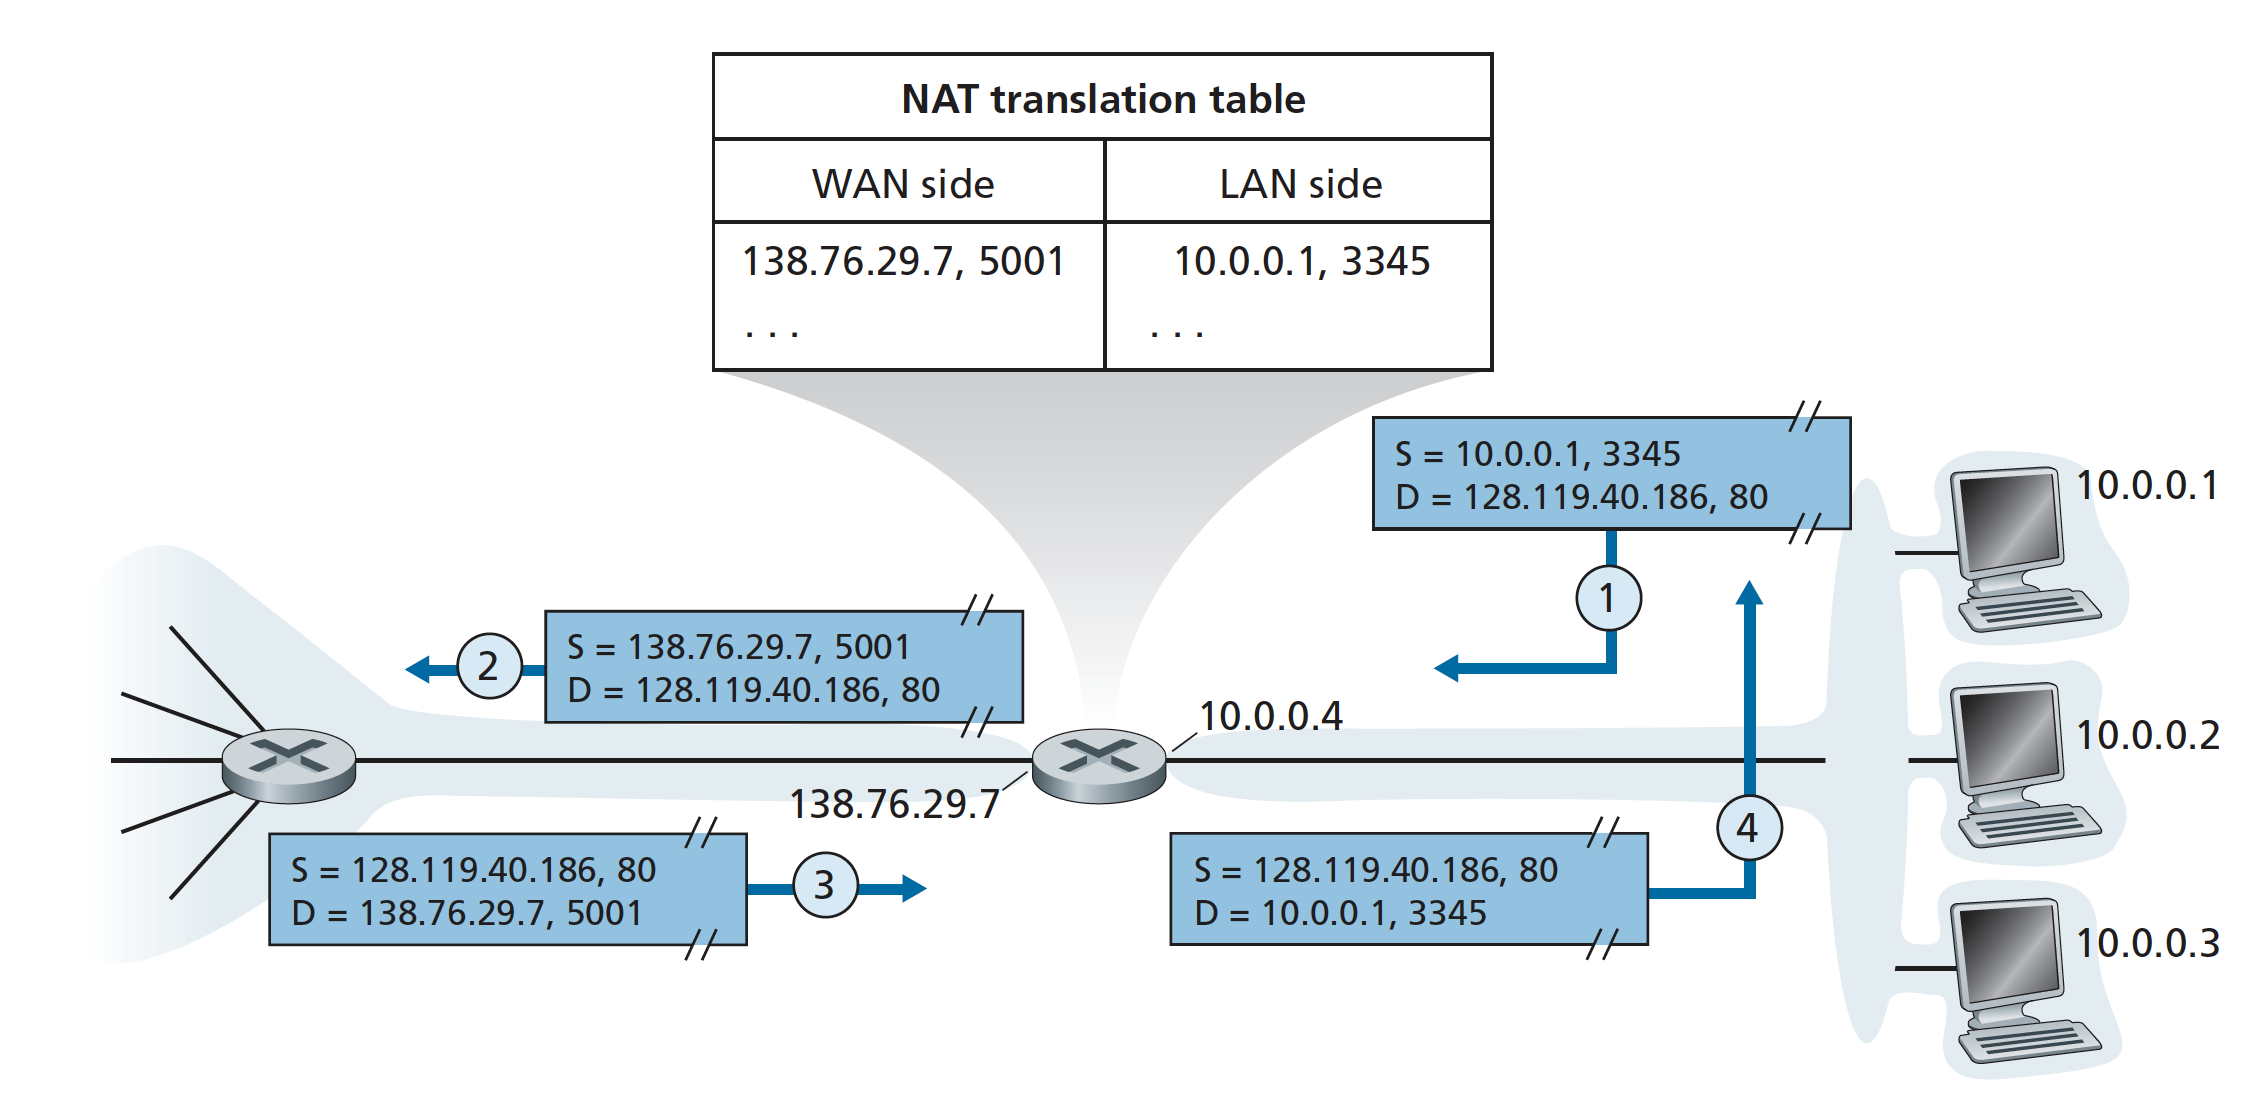
\includegraphics[keepaspectratio, width=15cm, height=12cm]{imagens/13/13 - NAT.png}
\caption{NAT \\
Imagem retirada de: Computer Networking a top-down approach. 8th
ed.~Pearson, página 345. \\}
\label{NAT}
\end{figure}





Um roteador com o protocolo NAT ativo é visto como um dispositivo único
(com o IP único) para o resto do mundo, escondendo, assim, os detalhes
das configurações de uma rede doméstica para as redes externas.

É interessante notar que o roteador obtém o endereço de IP via o
servidor DHCP oriundo do ISP (\emph{Internet Service Provider}). E por
sua vez, oferece um servidor DHCP para a sua sub-rede.

O segredo para o funcionamento do NAT está no \emph{NAT translation
table}.

Quando uma requisição é disparada por um \emph{host} para um
\emph{server} fora da rede, o roteador converte o endereço de IP de
origem para o seu, e gera uma nova porta. Dessa forma, a \emph{NAT
translation table} é populada, no lado WAN (rede do ISP), com endereço
de IP do roteador e porta gerada, e no lado LAN (rede doméstica),
endereço de IP do \emph{host} e porta da \emph{Thread}.

Por exemplo:

\begin{enumerate}
\def\labelenumi{\arabic{enumi}.}
\tightlist
\item
  \emph{Host} dispara um \emph{datagram} com origem 10.0.0.1 e porta
  3345 para o \emph{server} 128.119.40.186 porta 80.
\item
  O roteador gera uma nova porta e substitui os parâmetros de origem
  para essa porta gerada e para o seu endereço de IP (que por sua vez
  foi gerado pelo ISP). E registra essa conversão no \emph{NAT
  translation table}.
\item
  O \emph{server} recebe o \emph{datagram} com os parâmetros de origem
  do roteador, e o responde.
\item
  O roteador converte os parâmetros de destino utilizando a tabela NAT,
  e, por fim, direciona o \emph{datagram} recebido ao \emph{host}.
\end{enumerate}

Esse registro é mantido até o fim da conexão. Como o tamanho do campo
porta é de 16 bits, o protocolo NAT suporta mais de 60 mil conexões com
somente um único \emph{IP address}.

Um dos problemas causados por esses protocolos (DHCP e NAT) é referente
aos \emph{Home Servers}, pois como um servidor espera por uma requisição
de um \emph{client}, como esse \emph{client} pode saber qual é o atual
endereço de IP do servidor ? Como funcionaria a arquitetura P2P ?
Soluções para esse problema incluem \emph{NAT transversal tools} {[}RFC
5389, RFC 5128{]}, algo que não será debatido nesse texto.

\hypertarget{ipv6-datagram}{%
\section{IPv6 datagram}\label{ipv6-datagram}}

Há uma série de mudanças introduzidas com o IPv6, mostrado na Figura \ref{IPV6 Datagram}:


\begin{figure}[h!]
\centering
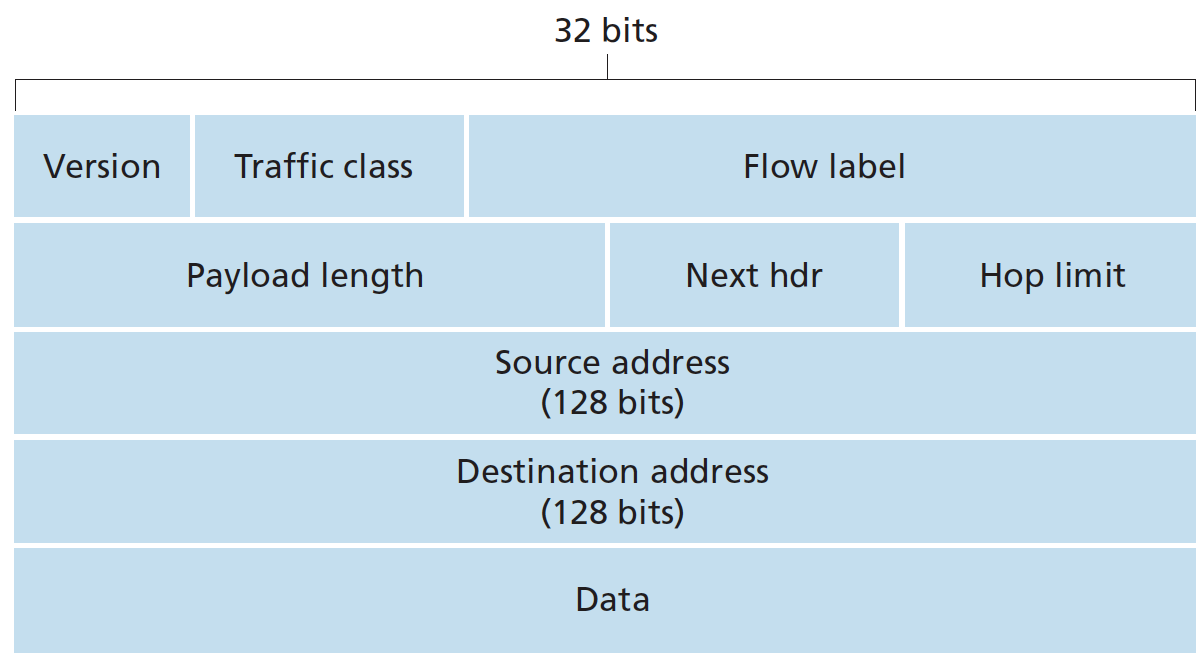
\includegraphics[keepaspectratio, width=12cm, height=9cm]{imagens/13/13 - IPv6 datagram.png}
\caption{IPV6 Datagram \\
Imagem retirada de: Computer Networking a top-down approach. 8th
ed.~Pearson, página 349. \\}
\label{IPV6 Datagram}
\end{figure}


\begin{enumerate}
\def\labelenumi{\arabic{enumi}.}
\tightlist
\item
  Capacidade de endereçamento expandido: de 32 bits para 128 bits
\item
  \emph{header} de tamanho fixo: o \emph{header} foi fixado em 40
  \emph{bytes}, permitindo um processamento mais rápido pelo roteador
\item
  fluxo e seu rótulo: capacidade de rotular os \emph{datagrams} de um
  fluxo específico, o qual cada rótulo sinaliza uma requisição
  específica, como \emph{real-time service} ou \emph{non-default
  quality}
\end{enumerate}

Os campos do \emph{datagram} do IPv6 são:

\begin{enumerate}
\def\labelenumi{\arabic{enumi}.}
\tightlist
\item
  Version: versão do IP (no caso, 6).
\item
  Traffic class: equivalente ao TOS do IPv4, é usado para dar prioridade
  à algum \emph{datagram}
\item
  \emph{flow label}: campo de 20 \emph{bits} usado para rotular um fluxo
  de \emph{datagrams}
\item
  \emph{Payload Length}: campo de 16 \emph{bits} que indica o tamanho do
  \emph{payload}
\item
  \emph{Next Header}: identifica o protocolo para qual o \emph{datagram}
  (ou o \emph{payload}) será entregue
\item
  \emph{Hop limit}: equivalente ao TTL do IPv4, diminui em 1 toda vez
  que o \emph{datagram} é transmitido por um roteador e descartado
  quando chega em 0.
\item
  Endereço de origem e destino: no formato de 128 \emph{bits}
\item
  \emph{Data}: também chamado de \emph{payload}, é o conteúdo
  encapsulado pelo protocolo.
\end{enumerate}

Foram removidos:

\begin{enumerate}
\def\labelenumi{\arabic{enumi}.}
\tightlist
\item
  Fragmentação e remontagem: IPv6 não permite a fragmentação e a
  remontagem do datagram (essa operação era feita com o objetivo de
  reduzir o tamanho do \emph{datagram} grande demais para ser
  transmitido). Assim caso um \emph{datagram} seja muito grande, o
  roteador descarta esse \emph{datagram} e retorna uma mensagem de erro,
  de forma que o emissor deverá reenviar o \emph{datagram}. A remoção
  dessa funcionalidade gera, como resultado, uma redução no tempo de
  processamento do roteador.
\item
  \emph{Header checksum}: Considerado suficientemente redundante e
  enfatizando a velocidade de processamento, esse campo não se mostrou
  necessário para os desenvolvedores do IPv6.
\item
  Options: a remoção do \emph{options} possibilitou a fixação do tamanho
  do \emph{header} em 40 \emph{byts}, algo que além de causar um
  encolhimento no tempo de processamento, também deixa explícito o
  início do \emph{payload} (afinal, o \emph{payload} sempre estará 40
  bytes após o início do \emph{datagram}).
\end{enumerate}

\hypertarget{transiuxe7uxe3o-de-ipv4-para-ipv6}{%
\section{Transição de IPv4 para IPv6}\label{transiuxe7uxe3o-de-ipv4-para-ipv6}}

Há um problema inerente na atualização dos sistemas distribuídos: a
adoção de uma nova tecnologia por todos os elementos da rede Um sistema
com o IPv6 pode ser projeto para ser retro-compatível com o IPv4, mas um
sistema com IPv4 não é capaz de lidar com o IPv6.

Como, então, atualizar todos os incontáveis dispositivos já integrados
na rede ?

\begin{enumerate}
\def\labelenumi{\arabic{enumi}.}
\tightlist
\item
  Transição abrupta: substituir todos os elementos de uma vez só,
  marcando um dia x para inutilizar os dispositivos compatíveis com
  IPv4.
\item
  Transição suave: substituir os elementos de forma gradual.
\end{enumerate}

A abordagem da transição suave foi o caminho escolhido. Para tal, fora
adotado a prática do \emph{tunneling} (algo que torna os dispositivos
IPv6 compatível com o IPv4). O \emph{tunnel} encapsula o \emph{datagram}
do IPv6 integralmente, tornando-o o \emph{payload} do IPv4, resultando
em um \emph{datagram} com o \emph{header} do IPv4 (como mostrado na Figura \ref{Tunneling}).


\begin{figure}[h!]
\centering
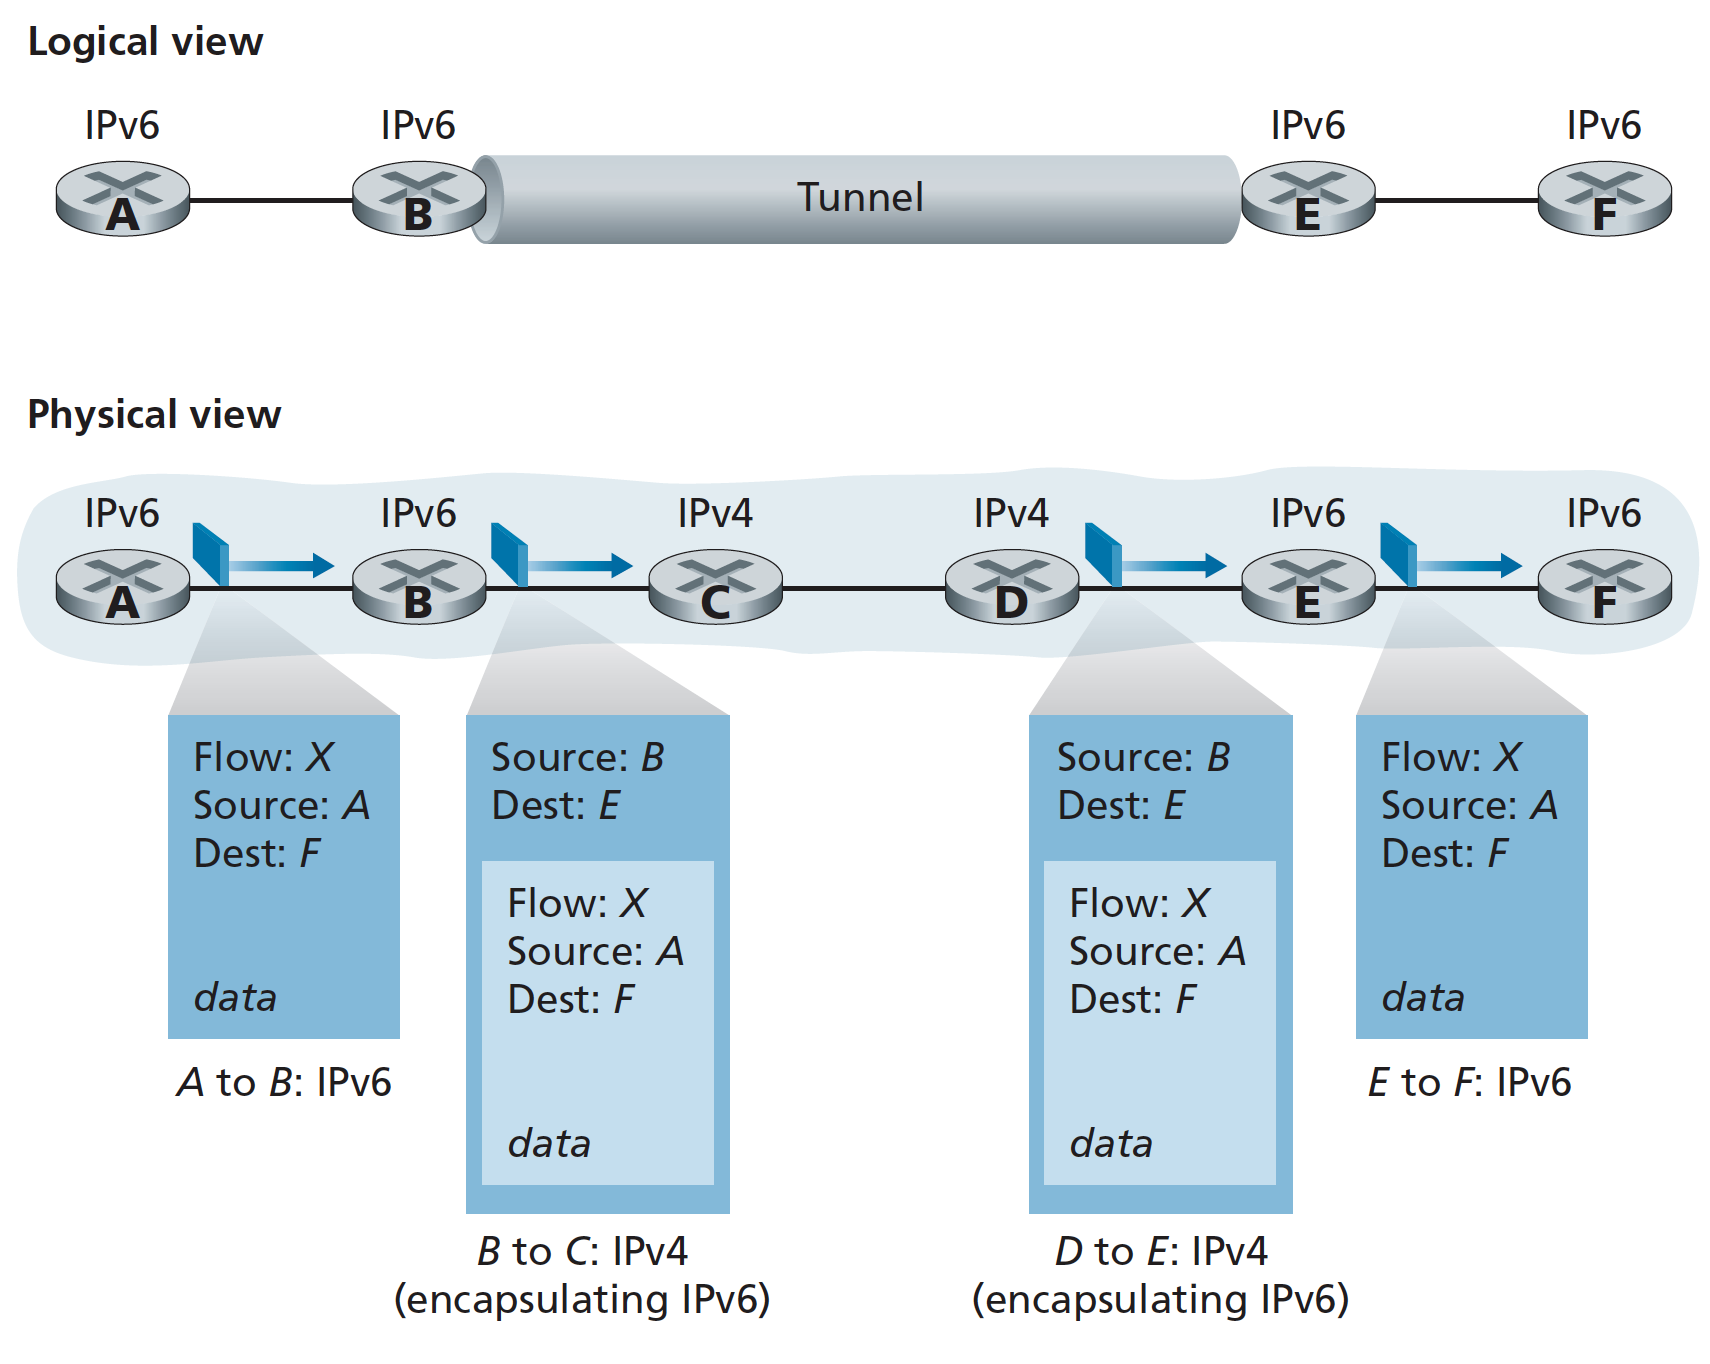
\includegraphics[keepaspectratio, width=14cm, height=11cm]{imagens/13/13 - Tunneling.png}
\caption{Tunneling \\
Imagem retirada de: Computer Networking a top-down approach. 8th
ed.~Pearson, página 352. \\}
\label{Tunneling}
\end{figure}



\hypertarget{link-layer}{%
\chapter{Link Layer}\label{link-layer}}

Após a \emph{Network Layer} determinar qual o caminho de comunicação
(chamado de \emph{link} ou enlace) o \emph{datagram} deve percorrer, como
o \emph{WiFi} ou o \emph{Ethernet}, entra em cena o \emph{Link Layer}
(camada de enlace), responsável por encapsular o \emph{datagram} e
transmitir o resultado (o \emph{frame}) através do \emph{link}. Os
dispositivos que executam a camada de enlace são chamados de nós
(\emph{nodes}).

Fundamentalmente, os \emph{links} podem ser classificados em dois canais
de comunicação. O primeiro refere-se aquele no qual os nós compartilham
do mesmo caminho de transmissão (\emph{single broadcast link}), como os
\emph{wireless LANs}. O segundo tipo é de ponto-a-ponto, no qual somente
dois nós são conectados em cada \emph{link}.

O \emph{link layer} está presente tanto em \emph{software} (com, por
exemplo, a montagem das informações de endereçamento e o controle de
interrupções) como em \emph{hardware} (com, por exemplo, \emph{link
access} e \emph{framing}) e é implementado em um \emph{chip} chamado de
\emph{Network Interface Controller} (NIC).

\hypertarget{serviuxe7os}{%
\section{Serviços}\label{serviuxe7os}}

A camada de enlace provê os seguintes serviços:


\begin{enumerate}
\def\labelenumi{\arabic{enumi}.}
\tightlist
\item
  \emph{Framing}: constituição do \emph{frame} a partir do
  encapsulamento do \emph{datagram}.
\item
  \emph{Link access}: o controle de acesso é algo fundamental para a
  realização da transmissão, sendo esse realizado pelo \emph{Medium
  Access Protocol} (MAC protocol). Nos \emph{links} ponto-a-ponto, o
  protocolo somente verifica se o \emph{link} está disponível. Em
  \emph{single broadcast link}, ocorre o problema de multiplos acessos
  simultâneos, sendo da responsabilidade do protocolo MAC especificar as
  regras para a transmissão dos \emph{frames}
\item
  \emph{Reliable delivery}: protocolo que objetiva garantir a transmissão
  de cada \emph{datagram}.
\item
  \emph{Error detection and corretion}: devido à possíveis erros
  introduzidos pela atenuação do sinal ou ruídos eletromagnéticos,
  vários protocolos fornecem mecanismos de detecção e correção de erros.
\end{enumerate}

\hypertarget{endereuxe7amento-o-switches}{%
\section{Endereçamento}\label{endereuxe7amento-o-switches}}

O \emph{Link Layer} utiliza um sistema de endereçamento similar ao
\emph{Network Layer} com o \emph{IP Address}.

Na fabricação de um NIC, lhe é designado um endereço único de 6 bytes
chamados de \emph{MAC Address} (\emph{LAN Address}, ou \emph{Physical
Address}), que se complementa ao \emph{IP Address} de forma similar à
relação entre o CPF de um brasileiro com seu endereço residencial, pois
o endereço residencial é alterado conforme ocorre uma mudança (assim
como o \emph{IP Address} é alterado após o dispositivo mudar de rede),
mas o seu CPF não é modificado (assim como o \emph{MAC Address}).
Portanto, é designado (pelo fabricante) ao NIC um \emph{MAC Address}, e
(pela rede) um \emph{IP Address}.

\hypertarget{arp}{%
\subsection{ARP}\label{arp}}

O \emph{Link Layer} necessita, para o envio de seus \emph{frames}, o
endereço MAC do dispositivo receptor. Mas como obter esse endereço ?
Esse endereço pode ser obtido através do \emph{Address Resolution
Protocol} (ARP), no qual armazena em uma tabela (ARP \emph{table}) as
equivalências entre \emph{IP Address} e \emph{MAC Address}. A ARP
\emph{table} está localizada nos NICs de cada \emph{host} e
\emph{router} da sub-rede.

O ARP é similar ao DNS, com a diferença de estar limitado à sua sub-rede
(diferente do DNS que está disponível para toda a Internet).

\hypertarget{funcionamento-do-arp}{%
\subsubsection{Funcionamento do ARP}\label{funcionamento-do-arp}}

Suponha que o \emph{host} 222.222.222.220 quer enviar um \emph{datagram}
para 222.222.222.222, mas não tenha em sua ARP \emph{table} o registro
contendo a equivalência entre o IP e o MAC \emph{Address}. Para tal, o
emissor deve utilizar o protocolo ARP:

\begin{enumerate}
\def\labelenumi{\arabic{enumi}.}
\tightlist
\item
  O emissor deve inquerir (\emph{query}) todos os \emph{hosts} e
  \emph{routers} da sub-rede para determinar a equivalência. Esse
  inquérito ocorre com a montagem de um ARP \emph{packet} (uma estrutura
  especial que contém o endereço IP e MAC do emissor e do receptor)
  destinado ao \emph{MAC Broadcast Address} (um endereço específico,
  FF-FF-FF-FF-FF-FF, no qual sinaliza que a transmissão deve ser feito
  para todos os \emph{hosts} da sub-rede)
\item
  O NIC encapsula o ARP \emph{packet} em um \emph{link layer frame} e
  transmite para a sub-rede (equivalente a uma pessoa gritar em uma sala
  quem tem um CPF XXX.XXX.XXX-XX)
\item
  O \emph{host} no qual o seu módulo ARP contém o registro inquerido
  envia de volta (diretamente ao inquisidor) um \emph{response} ARP
  \emph{packet} com o mapeamento desejado.
\item
  O \emph{host} inquisidor, por fim, pode atualizar sua ARP \emph{table}
  e enviar os seus dados para o endereço MAC correspondente à
  inquisição.
\end{enumerate}

É importante perceber que: 1. O \emph{query} ARP \emph{message} é
enviado para todos em \emph{broadcast}, enquanto que sua resposta não
(ela é enviada em um \emph{frame} padrão). 2. ARP é
\emph{plug-and-play}, montando sua tabela automaticamente. 3. O ARP é um
protocolo localizado entre o \emph{Network Layer} e o \emph{Link Layer},
por conter parâmetros oriundos de ambas as camadas (como o \emph{IP
Address} e o MAC \emph{Address}, respectivamente) 4. O ARP opera quando
um \emph{host} quer enviar um \emph{datagram} para outro \emph{host} na
mesma sub-rede.

Como um emissor pode enviar um \emph{datagram} para fora de sua rede se
o MAC \emph{Address} de destino é necessário e o protocolo ARP não
fornece o endereço de dispositivos fora da sub-rede ?

A resposta: Não é necessário que o emissor saiba do MAC \emph{Address} do
\emph{host} de destino ! Basta o emissor popular o campo MAC
\emph{Address} de destino com o MAC \emph{Address} do roteador da sua
rede! (Que pode ser obtido pelo ARP)

O roteador da rede do emissor receberá o \emph{datagram} e avaliará para
qual NIC esse \emph{datagram} deve ser direcionado (isso é feito
consultando o \emph{fowarding table}). Uma vez no NIC (da sub-rede 2), o
módulo ARP é acionado para obter o MAC \emph{Address} do destinatário.
Por fim, o \emph{datagram} é encapsulado pelo \emph{Link Layer} e
transmitido para o receptor da mensagem.

\hypertarget{ethernet}{%
\section{Ethernet}\label{ethernet}}

O protocolo \emph{Ethernet} foi inventado nos anos 1970 por Bob Metcalfe
e David Boggs. Inicialmente utilizava um barramento coaxial (uma
\emph{broadcast} LAN) para interconectar os nós. Os padrões utilizados
eram os 10BASE-2 e 10BASE-5 (10 refere-se à velocidade, em Mbps, BASE ao
\emph{baseband} Ethernet, significando que a mídia física só carrega o
tráfico de dados Ethernet, e a parte final refere-se a mídia física em
si, como o cabo coaxial), os quais especificavam 10Mbps Ethernet em
cabos coaxiais limitados a 500 metros. Distâncias maiores poderiam ser
obtidas com o uso dos \emph{repeaters}, dispositivos da camada física
que repetem o sinal de entrada na sua saída.

Em 1990, os barramentos coaxiais foram substituídos pelo cabo de cobre
de par trançado conectado em um Hub, um dispositivo da camada física
(\emph{1-layer}) que retransmite os bits de entrada para todos os nós
conectados a ele, em uma arquitetura estrela (com todos os \emph{hosts}
conectados ao dispositivo central, o Hub), mantendo-se, portanto, uma
\emph{broadcast} LAN. Um problema presente nos \emph{Hubs} ocorre quando
múltiplos \emph{frames} são transmitidos simultaneamente, algo que gera
uma colisão, e os nós que criaram os \emph{frames} devem
retransmiti-los.

A solução para as colisões veio nos anos 2000, quando o \emph{Hub} fora
substituído pelo \emph{Switch}, dispositivo de segunda camada
(\emph{2-layer}, camada de enlace) que armazenam e transmitem
(\emph{store-and-foward}) os dados utilizando o \emph{MAC Address} para
direcioná-los aos seus respectivos \emph{links}, tornando, assim,
dispensável o uso do protocolo MAC (protocolo para controle de colisão).

O \emph{Ethernet} tornou-se o protocolo dominante em redes LAN
(\emph{Local Area Network}) por:

\begin{enumerate}
\def\labelenumi{\arabic{enumi}.}
\tightlist
\item
  Ser o primeiro a implantar largamente o \emph{high-speed} LAN
\item
  Era mais simples e barato do que seus concorrentes
\item
  \emph{Data rates} compatíveis ou maiores do que os seus concorrentes
\item
  Por consequência de sua popularidade, dispositivos \emph{Ethernet} são
  mais baratos.
\end{enumerate}

É importante perceber que, apesar da intensa mudança de padrão sofrida
desde os anos 1970, o Ethernet ainda utiliza a mesma estrutura de
\emph{frame}, algo que será debatido posteriormente.

\hypertarget{ethernet-frame}{%
\subsection{Ethernet Frame}\label{ethernet-frame}}

O \emph{frame} do Ethernet, como mostrado na Figura \ref{Estrutura do frame Ethernet}, é composto por:


\begin{figure}[h!]
\centering
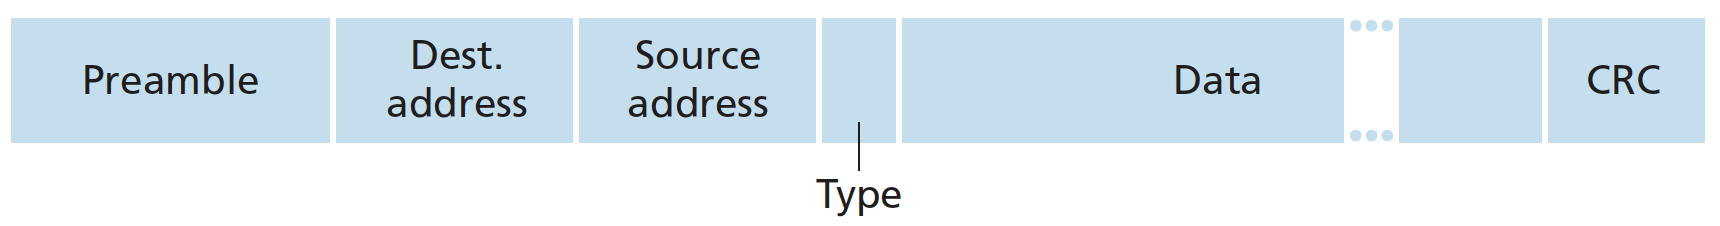
\includegraphics[keepaspectratio, width=12cm, height=9cm]{imagens/13/13 - estrutura do frame ethernet.png}
\caption{Estrutura do frame Ethernet \\
Imagem retirada de: Computer Networking a top-down approach. 8th
ed.~Pearson, página 486. \\}
\label{Estrutura do frame Ethernet}
\end{figure}


\begin{enumerate}
\def\labelenumi{\arabic{enumi}.}
\tightlist
\item
  \emph{Data Field} (\emph{payload}): é o local no qual é carregado o
  \emph{datagram} (resultado da camada superior). Tem o tamanho máximo
  (\emph{Maximum Transmission Unit}, MTU) de 1500 \emph{bytes} e mínimo
  de 46 \emph{bytes}. Caso o \emph{datagram} seja maior, o \emph{host}
  deve fragmentá-lo. Caso seja menor, o campo \emph{Data Field} é
  preenchido (\emph{stuffed}) até o mínimo (o campo \emph{length}
  presente no \emph{header} do \emph{datagram} indicará o seu tamanho
  correto).
\item
  \emph{Destination Address}: Esse campo contém o MAC \emph{Address} de
  destino (endereço de 6 bytes).
\item
  \emph{Source Adress}: Esse campo contém o MAC \emph{Address} de origem
  da mensagem (endereço de 6 bytes).
\item
  \emph{Type Field} (2 \emph{bytes}): Indica o protocolo utilizado no
  \emph{datagram} (como IP e ARP).
\item
  \emph{Cycic redundancy check} (CRC) (4 \emph{bytes}): permite o
  receptor identificar erros no \emph{frame}.
\item
  \emph{Preamble} (8 bytes): o \emph{frame} inicia com o
  \emph{preamble}. É utilizado para ``acordar'' o NIC receptor e
  sincronizar os seus relógios.
\end{enumerate}

O Ethernet é \emph{conectionless} ou seja, não requer de
\emph{handshaking} anterior ao envio de uma mensagem. Após enviado uma
mensagem, não há respostas confirmando sua chegada
(\emph{acknoledgments}). Assim, seu serviço é dito como não confiável,
algo que torna o Ethernet simples e barato.

\hypertarget{switch}{%
\section{Switch}\label{switch}}

O \emph{Switch} é transparente para os dispositivos da sub-rede (os
dispositivos não sabem da presença do \emph{switch}), e seu princípio de
funcionamento (\emph{match plus action}) é baseado no \emph{Filtering
and Fowarding}, no qual o \emph{Filtering} determina se um \emph{frame}
deve ser descartado ou transmitido, e o \emph{Fowarding} define qual
interface o \emph{frame} deve ser transmitido. O \emph{Filtering and
Fowarding} utiliza uma tabela chamada de \emph{switch table}, a qual
armazena registros com os campos \emph{address}, referente ao MAC
\emph{Address}, \emph{Interface}, indicando qual interface o endereço
MAC está anexado, e \emph{Time}, que marca o tempo no qual o registro
fora armazenado.

Existem 3 casos para o \emph{Filtering and Fowarding}:

\begin{enumerate}
\def\labelenumi{\arabic{enumi}.}
\tightlist
\item
  Não há registro para o MAC \emph{Address} de destino: dispara para
  todos os dispositivos (\emph{broadcast}).
\item
  O MAC \emph{Address} de destino é o mesmo da interface no qual o
  \emph{frame} fora recebido: discarta o \emph{frame}
  (\emph{filtering}).
\item
  Há um registro referente ao MAC \emph{Address} de destino com a
  interface sendo diferente a da origem do \emph{frame}: põe o
  \emph{frame} no \emph{buffer} que corresponde à interface de destino
  (\emph{fowarding}).
\end{enumerate}

É interessante perceber que o \emph{switch} é \emph{self learning}
(aprende sozinho). Essa capacidade é obtida da seguinte forma:

\begin{enumerate}
\def\labelenumi{\arabic{enumi}.}
\tightlist
\item
  A \emph{switch table} inicializa vazia.
\item
  Para cada \emph{frame} recebido, o \emph{switch} armazena na sua
  tabela: o MAC \emph{Address} da origem; a interface no qual o
  \emph{frame} foi recebido; o tempo atual. Dessa maneira,
  eventualmente, o \emph{switch} preencherá completamente sua tabela.
\item
  Um registro é deletado caso não seja recebido \emph{frames} com o seu
  MAC \emph{Address} de origem após um certo período de tempo
  (\emph{aging time}).
\end{enumerate}

O \emph{switch} apresenta algumas vantagens sobre o \emph{hub}:

\begin{enumerate}
\def\labelenumi{\arabic{enumi}.}
\tightlist
\item
  Eliminação de colisões: não há perda no comprimento de banda por
  consequência das colisões.
\item
  \emph{Links} heterogêneos: os diferentes \emph{links} podem operar com
  velocidades e mídias diferentes.
\item
  Gerenciamento: além de melhorar a segurança, os \emph{switches}
  coletam estatísticas de rede que podem ser usados para melhorá-la.
\end{enumerate}

Em comparação com os roteadores, os \emph{switches} apresentam:

Vantagens:

\begin{enumerate}
\def\labelenumi{\arabic{enumi}.}
\tightlist
\item
  \emph{Plug-and-play}.
\item
  Altas taxas de \emph{filtering and fowarding}
\end{enumerate}

Desvantagens:

\begin{enumerate}
\def\labelenumi{\arabic{enumi}.}
\tightlist
\item
  Topologia de rede restrita
\item
  Suscetível ao \emph{broadcast storm}: caso um \emph{host} dispare
  incontáveis \emph{frames} em \emph{broadcast}, a operação do
  \emph{switch} pode saturar a rede, podendo colapsá-la.
\end{enumerate}

Roteadores:

Vantagens: 1. \emph{Datagrams not cycle}: mesmo com caminhos
redundantes, os \emph{datagrams} não se mantém vivos vagando pela rede
(proteção vinda de campos como TTL). 2. Topologia de rede não restrita
3. \emph{Firewall} contra \emph{broadcast storm} (não suscetível ao
\emph{broadcast storm}). 4. Provê um isolamento mais robusto

Desvantagens:

\begin{enumerate}
\def\labelenumi{\arabic{enumi}.}
\tightlist
\item
  Não é \emph{plug and play}
\item
  Maior tempo de processamento: pois os roteadores devem processar até a
  terceira camada.
\end{enumerate}